\documentclass{article}
\usepackage[italian]{babel}
\usepackage[tmargin=2cm,rmargin=1.5in,lmargin=1.5in,margin=0.85in,bmargin=2cm,footskip=.2in]{geometry}
\usepackage{siunitx}
\sisetup{separate-uncertainty=true, per-mode=fraction, parse-numbers=true}
\usepackage{caption}
\usepackage[T1]{fontenc}
\usepackage{bookmark}
\usepackage{graphicx}
\usepackage{multicol}
\usepackage{booktabs}
\usepackage{amsmath,amsfonts,amsthm,amssymb,mathtools}
\hypersetup{
	pdftitle={Appunti Tomadin},
	colorlinks=true, linkcolor=doc!90,
	bookmarksnumbered=true,
	bookmarksopen=true
}
\usepackage{blindtext}
\usepackage{wrapfig}
\usepackage{listings}
\usepackage{xcolor}
\usepackage{float}
\usepackage{tikz}
\usepackage{multirow}
\usepackage{biblatex}
\definecolor{codegreen}{rgb}{0,0.6,0}
\definecolor{codegray}{rgb}{0.5,0.5,0.5}
\definecolor{codepurple}{rgb}{0.58,0,0.82}
\definecolor{backcolour}{rgb}{0.95,0.95,0.92}
\definecolor{doc}{rgb}{0,0,0}
\lstdefinestyle{code}{
    backgroundcolor=\color{backcolour},   
    commentstyle=\color{codegreen},
    keywordstyle=\color{magenta},
    numberstyle=\tiny\color{codegray},
    stringstyle=\color{codepurple},
    basicstyle=\ttfamily\footnotesize,
    breakatwhitespace=false,         
    breaklines=true,                 
    captionpos=b,                    
    keepspaces=true,                                     
    showspaces=false,                
    showstringspaces=false,
    showtabs=false,                  
    tabsize=2,
    inputencoding=ansinew,
    extendedchars=true,
    numbers=left,                    
    numbersep=5pt
}

\lstset{style=code}
\usepackage[varbb]{newpxmath}
\usepackage{circuitikz}
\author{Aiello Giosuè, Fenili Domenico, Sermi Francesco}
\date{\today}
\title{Relazione conducibilità termica}

\begin{document}
\maketitle
\newpage

\tableofcontents

\newpage

\section{Scopo}

Ricavare la conducibilità termica di differenti materiali dalle misurazioni di temperatura compiute

\section{Premesse teoriche}

Dalla teoria sappiamo che la quantità di calore che si trasmette per conduzione nell'unità di tempo è pari a
\begin{equation}
	W = \frac{dQ}{dt}
\end{equation}
è detta \emph{flusso di calore} e nel sistema MKS si misura in \unit{W}. All'equilibrio termico si osserva che il flusso di calore che attraversa la barra risulta costante e, se denotiamo con $S$ la sezione della barra, $T$ la temperatura ed $x$ la posizione lungo la barra; abbiamo che:
\begin{equation}
	W = -\lambda S \frac{\Delta T}{\Delta x}
\end{equation}
dove la costante di proporzionalità $\lambda$ viene detta \emph{conducibilità termica} del materiale. Se fissiamo l'origine delle ascisse in $x_0$, abbiamo che
\begin{equation}
	W = -\lambda S \frac{T_i - T_0}{x_i}
\end{equation}
ovvero
\begin{equation}
	T_i = T_0 - \frac{W}{\lambda S}x_i
\end{equation}
Sappiamo inoltre che, per effetto Joule, la potenza dissipata come calore è pari a
\begin{equation}
	W = VI
\end{equation}
Per calcolare la conducibilità sfrutteremo il fatto che, ipotizzando l'assenza di perdite, vale la relazione
\begin{equation}
	T_i = T_0 - \frac{VI}{2 \lambda S}x_i
	\label{eq:modello}
\end{equation}
dove poniamo che $W$ sia pari a $\frac{VI}{2}$ siccome stiamo operando con un circuito con due termistori uguali in parallelo.

\section{Strumenti e materiali utilizzati}

\textbf{Materiali:}
\begin{itemize}
	\item Due barre cilindriche;
	\item Un circuito di acqua corrente;
	\item Generatore di corrente continua con display per visualizzare la differenza di potenziale e l'intensità di corrente emessa;
	\item Un alimentatore chiuso su due resistenze in parallelo;
\end{itemize}
\textbf{Strumenti:}
\begin{itemize}
	\item Calibro ventesimale, con sensibilità pari a $\pm 0.005 cm$
	\item Due termistori per la misura della temperatura;
	\item Calcolatore con programma di acquisizione;
	\item Scheda Arduino;
	\item Calibro per misurare le distanze e la sezione
\end{itemize}
\section{Descrizione delle misure}

Per effettuare questa esperienza, dovevamo misurare le temperature $T_i$ di una serie di punti all'interno di due sbarre di diverso materiale a noi sconosciuto. \\
Prima di procedere con le misurazioni abbiamo misurato dal generatore di corrente continua la differenza di potenziale che veniva emessa dal circuito costituito dalle due resistenze in parallelo e l'intensità di corrente elettrica, riportate qua sotto:
\begin{align*}
	&V = (10.2 \pm 0.1) \, \text{\unit{V}} \\
	&i = (1.65 \pm 0.01) \, \text{\unit{A}}
\end{align*}
e abbiamo inoltre misurato il diametro delle due rispettive sbarre, pari a:
\begin{align*}
	&l_1  = (25.00 \pm 0.05) \, \unit{mm} \\
	&l_2  = (25.20 \pm 0.05) \, \unit{mm}
\end{align*}

\begin{wraptable}{l}{0.3\textwidth}
\centering
\begin{tabular}{c c} \toprule
$T_0$ ($s$) & $T_1$ ($s$) \\
$\pm 0.01$ & $\pm 0.01$ \\ \toprule
49.75 &	48.79 \\ \midrule
49.61 &	48.79 \\ \midrule
49.61 &	48.79 \\ \midrule
49.61 &	48.79 \\ \midrule
49.75 &	48.79 \\ \midrule
49.61 &	48.79 \\ \midrule
49.61 &	48.79 \\ \midrule
49.75 &	48.79 \\ \midrule
49.75 &	48.79 \\ \midrule
49.61 &	48.79 \\ \midrule
49.75 &	48.79 \\ \bottomrule
\end{tabular}
\captionof{table}{Tabelle con un esempio di alcune misurazioni: la temperatura $T_0$ è la temperatura misurata del primo termistore che mantenevamo fisso nel primo buco (siccome la sbarra non era in equilibrio termico e dovevamo tenere conto di questa variazione) e la temperatura $T_1$ è la temperatura misurata dal secondo termistore}
\end{wraptable}

\noindent Per fare queste misurazioni ci siamo avvalsi di un calcolatore con un programma di acquisizione che si collegava, tramite una serie di librerie ad hoc, alla scheda di acquisizione con Arduino a cui erano collegati i termistori: i materiali, di cui noi dovevamo calcolare la conducibilità termica, possedevano vari buchi dove noi mettevamo entrambi  i termistori per misurare, attivando il processo di lettura dal programma predisposto per questa esperienza sul calcolare, per far misurare i valori di temperatura alla scheda di Arduino che campionava il valore ogni $0.5 \ s$ circa. \\
Siccome la barra man mano che si procedeva con l'esperimento si riscaldava sempre di più, noi abbiamo mantenuto un termistore nel primo buco che avevamo, in maniera tale da misurare continuamente la temperatura $T_0$. \\
Riporto una tabella d'esempio per mostrare in che forma si presentavano i dati raccolti qua di fianco, qua di lato (precisamente, i dati qua mostrati sono alcuni quelli misurati a $\Delta x = 4.26 \pm 0.01 \, \unit{cm}$)
\section{Analisi delle misure}
Facendo riferimento all' equazione~\ref{eq:modello} e denotando con $m = -\frac{VI}{2 \lambda S}$, utilizziamo il metodo del parametro libero del fit rispetto a $m$ per calcolarci indirettamente la conducibilità termica del materiale $\lambda$ tramite la seguente relazione
\begin{equation}
	\lambda = \frac{VI}{2mS} \label{eq:lambda}
\end{equation}
da cui possiamo poi confrontare con il valore reale aspettato.
Per analizzare questi dati abbiamo, quindi, creato il grafico delle differenze di temperatura in funzione della differenze fra due punti $x_0$ (che nelle analisi abbiamo mantenuto fissato) e $x_1$ (che si faceva variare) del materiale. \\
Siccome la temperatura $T_0$ aumentava nel tempo (poiché non aveva ancora raggiunto l'equilibrio termico con la sorgente di calore) noi, rispetto a quanto detto nelle premesse teoriche, considereremo una \emph{variazione} della formula proposta sopra, ovvero:
\begin{equation}
	T_i - T_0 = -\frac{W}{\lambda S}(x_i-x_0) \implies \Delta T = --\frac{W}{\lambda S}\Delta x_i
\end{equation}
quindi faremo il fit del delle differenze di temperature rispetto alla differenze di lunghezza. \\
Siccome il programma di acquisizione dei dati prendeva tante misure, abbiamo deciso che, per ogni file prodotto, si prendevano le ultime $n$ misure e se ne considerava la differenza fra la temperatura $T_0$, misurata dal primo termistore (quello che si teneva fisso), e la temperatura $T_1$, la cui posizione si faceva variare. Di queste differenze si considerava poi la media aritmetica. Introdurre una media pesata si è scartata per vari motivi: in primis, le ultime misure solitamente presentano oscillazioni quasi nulle, quindi tutte le misurazioni avrebbero quasi lo stesso \emph{peso}, ma poi, a priori, non sappiamo quantificare, siccome non conosciamo effettivamente la misura della temperatura del materiale in quel punto, il grado di precisione con cui abbiamo misurato. \\
Per fare ciò abbiamo realizzato un programma in Python in grado di estrarre i dati da ogni file di estensione \emph{.txt} da cui si prendeva la temperatura misurata dai due termistori e si considerava la differenza di queste due. Per semplificare meglio, riporto un esempio di analisi dei dati per chiarire meglio il tipo di interpolazioni che effettuavamo:

\begin{wraptable}{r}{0.5\textwidth}
	\centering	
	\begin{tabular}{c c c} \toprule
		$T_0$ ($s$) & $T_1$ ($s$) & $T_0 - T_1$ ($s$) \\
		$\pm 0.01$ & $\pm 0.01$   & $\pm 0.02$ \\ \toprule
		51.35 &  50.08 &  1.27 \\ \midrule
		51.35 &  50.08 &  1.27 \\ \midrule
		51.35 &  50.08 &  1.27 \\ \midrule
		51.20 &  50.08 &  1.12 \\ \midrule
		51.20 &  50.08 &  1.12 \\ \bottomrule
	\end{tabular}
	\captionof{table}{Esempio di estrapolazione dei nostri dati: di ogni file si consideravano gli ultimi dati, quelli più significati poiché in quelli il termistore misurava correttamente il valore della temperatura siccome deve giungere, nel punto in cui veniva inserito, ad uno stato di equilibrio termico con il materiale}
\end{wraptable}

\noindent Un discorso molto delicato è sicuramente l'assegnazione delle incertezze sulla temperatura: infatti si potrebbe pensare che, in questo caso, siccome abbiamo la misurazione ripetuta di un campione allora potremmo usare la formula della deviazione standard della media aritmetica
\begin{equation}
	\sigma_\mu = \sqrt{\frac{1}{n(n-1)} \sum_{k = 0}^{n} (x_k - \mu)^2}
\end{equation}
dove con $\mu$ indichiamo media dei dati. \\
Il problema di questo approccio è il fatto che disegnando il grafico con i relativi errori si osserva che questi sono enormemente sottostimati e il motivo di ciò può essere il fatto che nel nostro apparato sperimentale erano presenti troppe sorgenti di errori sistematici che non possono essere trascurati: in primis, la sbarra \emph{reale} ha delle dispersioni di energia (il che potrebbe anche spiegare il motivo per cui la maggior parte delle misure sono inferiori al valore teorico) e i due termistori possono subire delle fluttuazioni del valore da loro misurato a causa di come questi sono fatti (e ad eventuali difetti di fabbricazione) e per il fatto che probabilmente i termistori con cui avevamo fatto non fossero dei termistori di precisione.


\begin{wrapfigure}{r}{0.5\textwidth}	
	\vspace{-1cm}
	\centering
	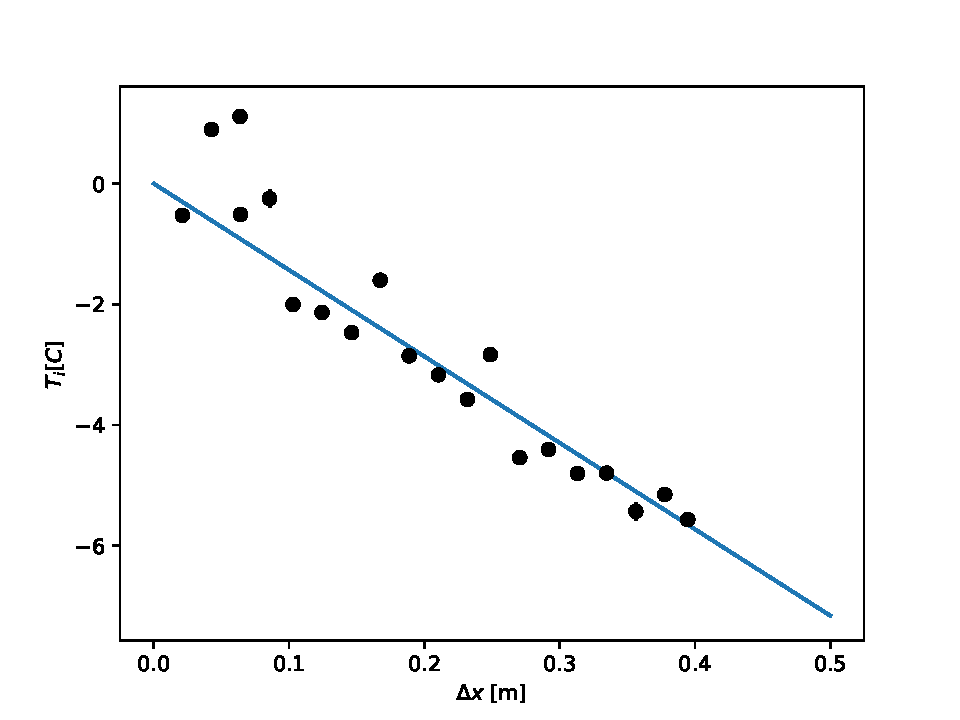
\includegraphics[scale=0.4]{Grafico_differenza_temperatura_rame_dev_scaled.pdf}
	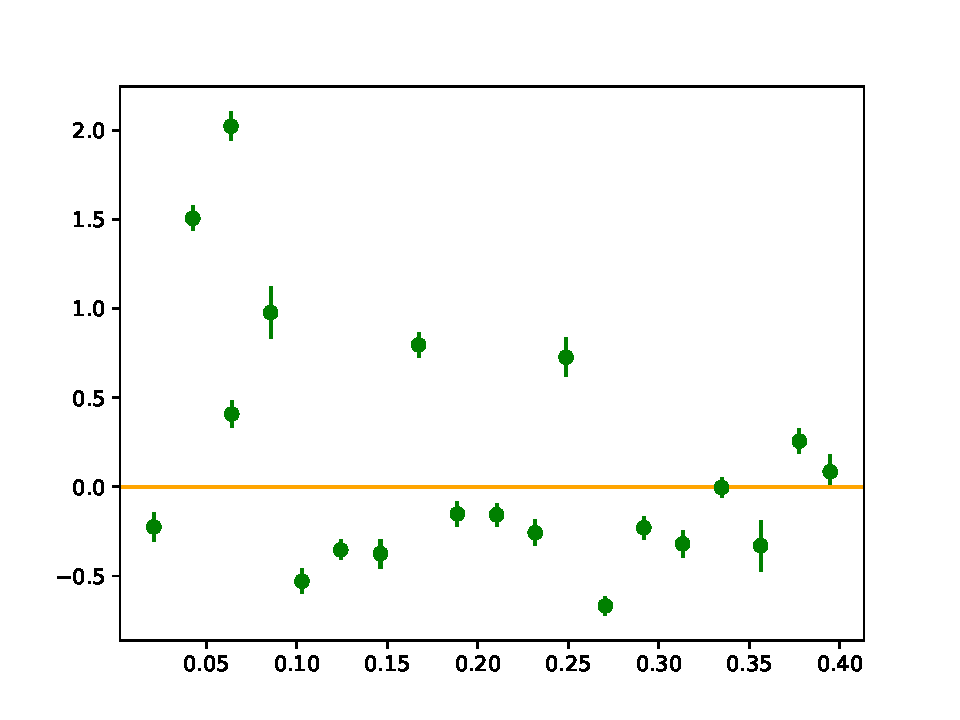
\includegraphics[scale=0.4]{Grafico_residui_rame_dev_scaled.pdf}
	\captionof{figure}{Immagine dei nostri grafici in cui si utilizza la deviazione della media aritmetica per stimare le incertezze sulla media delle differenze di temperatura: gli errori sono troppo \emph{piccoli} (fatto che è un evidente sintomo di una stima patologica che sottostima l'incertezza effettiva) e, nel caso specifico di questa immagine, abbiamo moltiplicato di un fattore $4$ gli errori per poterli farli vedere nell'immagine (e nel grafico $\Delta T \, - \, \Delta x$ rimangono comunque poco visibili)}
\end{wrapfigure}


Sebbene questi dati non siano statisticamente indipendenti, si potrebbe comunque procedere ad effettuare il fit (che, pur venendo meno l'ipotesi di indipendenza statistica fra i dati, può essere ragionevole in parte). Il $\chi^2$ con questi dati tuttavia risulta essere spropositato, infatti
\begin{equation*}
	\chi^2 \approx 26860
\end{equation*}
che è un valore troppo alto per i gradi di libertà del nostro esperimento. Inoltre, si osserva dal grafico dei residui che i valori non oscillano attorno allo zero, quindi, anche se trovassimo un modo per stimare in maniera più accurata gli errori presenti sulle nostre misure, i residui sono una prova inattaccabile della presenza di errori sistematici che non possono essere ignorati e mina la validità dell'operazione di \emph{fitting}. \\
Supponendo comunque che le stime effettuate dal fit possano essere comunque ragionevoli e avendo la stima del coefficiente angolare tramite \emph{scipy} della retta $\hat{m}$ legato alla conducibilità tramite la (\ref{eq:lambda}) abbiamo propagato l'errore su $\lambda$ nella seguente maniera
\begin{equation*}
	\sigma_\lambda = \lambda * \sqrt{ \left( \frac{\sigma_V}{V} \right)^2 + \left( \frac{\sigma_i}{i} \right)^2 + \left( \frac{\sigma_{\hat{m}}}{\hat{m}} \right)^2 + 4 \left(\frac{\sigma_r}{r} \right)^2} 
\end{equation*}
da cui si ricava che
\begin{equation*}
	\lambda = (3.0 \pm 0.2) * 10^2
\end{equation*}
\clearpage

che rispetto al valore atteso (sapendo che la conducibilità del rame è $~400 \, \unit{W/m^{-1}°C^{-1}}$) dista circa $5\sigma_{\lambda}$. Sebbene disti relativamente tanto dal valore teorico, potrebbe essere un valore quasi ragionevole considerando tutte le possibili fonte di dissipazioni presenti nella nostra strumentazione. \\
Passiamo adesso all'analisi dei dati dell'alluminio: questi, così come quelli del rame, soffrono sempre il medesimo problema riguardo le incertezze: osservando i grafici (riportati qua sotto a sinistra) si osserva che, usando la deviazione standard della media, se non fosse per qualche misurazione, avremmo dei dati abbastanza ragionevoli, 

\begin{wrapfigure}{l}{0.4\textwidth}
	\centering
	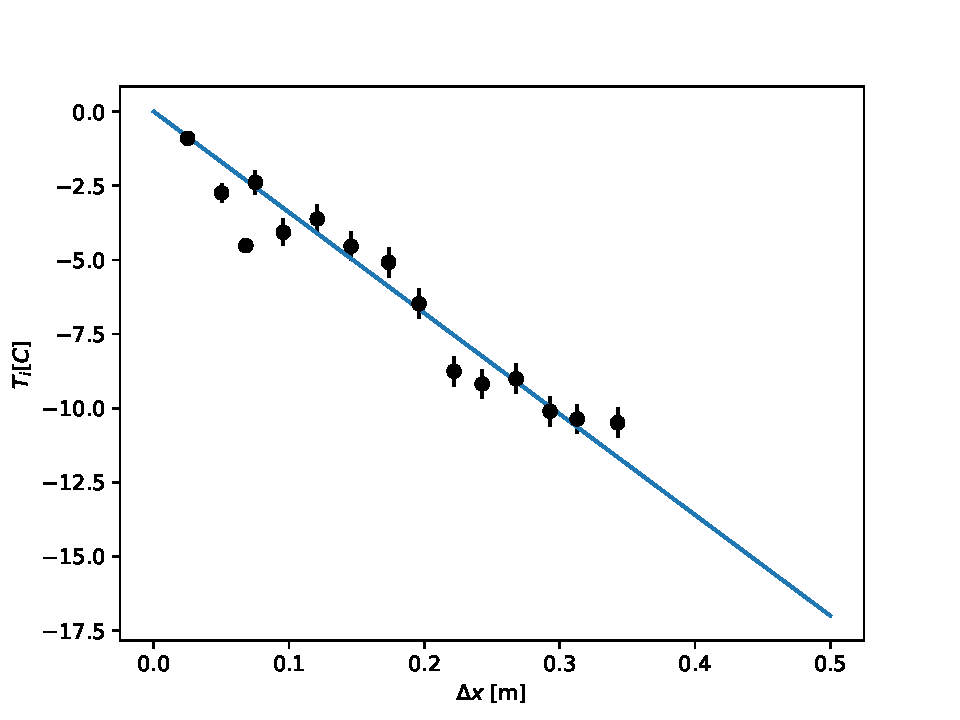
\includegraphics[scale=0.4]{Grafico_differenze_temperatura_alluminio_dev.pdf}
	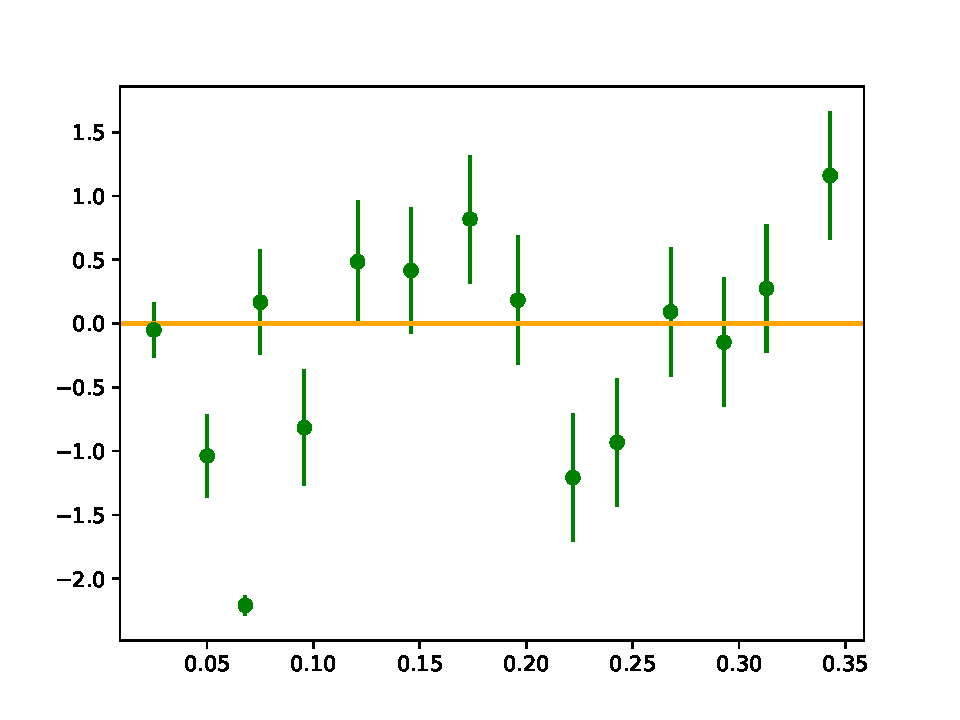
\includegraphics[scale=0.4]{Grafico_residui_alluminio_dev.pdf}
	\captionof{figure}{Immagine dei grafici e dei residui delle misurazioni effettuate }
\end{wrapfigure}

tuttavia, dal grafico dei residui si osserva che le nostre misure oscillano troppo poco attorno allo zero, il che ci porta a far ipotizzare che anche qua siano presenti errori sistematici, fatto avvalorato dal fatto che le misurazioni con il rame e con l'alluminio sono state effettuate con la stessa strumentazione e la stessa metodologia, pertanto è quasi certo che siano presenti le stesse sorgenti di errori sistematici.	\\
La stima del $\chi^2$ anche qua non produce un risultato molto apprezzabile, infatti risulta essere pari a
$$
	\chi^2 \approx 795
$$
che è spropositato rispetto ai gradi di libertà del fit. Osserviamo comunque la stima del coefficiente angolare della retta:
\begin{equation}
	m = (-33 \pm 1) \, \unit{°C/m}
\end{equation}
da cui, propagando l'errore come prima, si ottiene che la conducibilità termica è:
\begin{equation}
	\lambda = (126 \pm 5)
\end{equation}

\section{Conclusioni}

L'esperienza non può considerarsi un successo, siccome il risultato che abbiamo ottenuto si discosta di molto dal valore teorico, tuttavia è stata sicuramente un'esperienza istruttiva perché ci ha fatto fare i conti con gli errori sistematici.
\end{document}